%%%%%%%%%%%%%%%%%%%%%%%%%%%%%%%%%%%%%%%%%%%%%%%
% Template baseado no exemplo da classe utftex
% Prof. César M. V. Benítez
% DAELN, UTFPR-Curitiba (2019)
%%%%%%%%%%%%%%%%%%%%%%%%%%%%%%%%%%%%%%%%%%%%%%%

\documentclass[openright]{normas-utf-tex} %openright = o capitulo comeca sempre em paginas impares
%\documentclass[oneside]{normas-utf-tex} %oneside = para numero de paginas menor que 100 (apenas frente da folha) 

% force A4 paper format
\special{papersize=210mm,297mm}

\usepackage[alf,abnt-emphasize=bf,bibjustif,recuo=0cm, abnt-etal-cite=2, abnt-etal-list=99]{abntcite} %configuracao correta das referencias bibliograficas.

\usepackage[portuguese, ruled, linesnumbered]{algorithm2e}%pacotedealgoritmoemportugues

\usepackage[brazil]{babel} % pacote portugues brasileiro
\usepackage[utf8]{inputenc} % pacote para acentuacao direta
\usepackage{amsmath,amsfonts,amssymb} % pacote matematico
\usepackage{graphicx} % pacote grafico
\usepackage{times} % fonte times
\usepackage[final]{pdfpages} % adicao da ata
\usepackage[version=3]{mhchem}%adição de pacote para quimica
\usepackage{longtable}% redimensionar automaticamente tabelas
%\usepackage{hyperref}% link das res
\usepackage{array} % tamanho colunas tabelas
\newcommand\tab[1][1cm]{\hspace*{#1}}
%Podem utilizar GEOMETRY{...} para realizar pequenos ajustes das margens. Onde, left=esquerda, right=direita, top=superior, bottom=inferior. P.ex.:
%\geometry{left=3.0cm,right=1.5cm,top=4cm,bottom=1cm} 
\usepackage{amsthm}
\usepackage[hyphens]{url} %urls com hífens
\usepackage{subfig} % inclusao de subfiguras
\newtheorem{mydef}{Definicão}



\usepackage{listings}
\usepackage{xcolor}
\usepackage{color}
\definecolor{codegreen}{rgb}{0,0.6,0}
\definecolor{codegray}{rgb}{0.5,0.5,0.5}
\definecolor{codepurple}{rgb}{0.58,0,0.82}
\definecolor{backcolour}{rgb}{0.95,0.95,0.92}

\lstdefinestyle{mystyle}{
    backgroundcolor=\color{backcolour},   
    commentstyle=\color{codegreen},
    keywordstyle=\color{blue},
    numberstyle=\tiny\color{codegray},
    stringstyle=\color{orange},
    basicstyle=\ttfamily\footnotesize,
    breakatwhitespace=false,         
    breaklines=true,                 
    captionpos=b,                    
    keepspaces=true,                 
    numbers=left,                    
    numbersep=5pt,                  
    showspaces=false,                
    showstringspaces=false,
    showtabs=false,                  
    tabsize=2,
    morekeywords={True, False, self}
}

\lstset{style=mystyle}
%\usepackage{balance} 



% NOME DOS ALUNOS E PROFESSORES
\newcommand{\alunoA}{Anderson Nogueira Silva}
% \newcommand{\alunoB}{Nome Sobrenome B}
% \newcommand{\alunoC}{Nome Sobrenome C}
% \newcommand{\alunoD}{Nome Sobrenome D}

% Geralmente orientador e co-orientador
\newcommand{\professorA}{Laudelino Cordeiro Bastos}
% \newcommand{\professorB}{Nome Professor B}

% DISCIPLINA RELATIVA AO TRABALHO
\newcommand{\disciplina}{Engenharia de Requisitos}

% ---------- Preambulo ----------
\instituicao{UNIVERSIDADE TECNOLÓGICA FEDERAL DO PARANÁ (UTFPR)} % nome da instituicao
% \programa{NOME DO CURSO} % nome do programa de ensino (aparece abaixo do nome da instituição na capa)
\area{Engenharia de Computação} 
\documento{\disciplina} % Nome da disciplina relativa ao trabalho
\nivel{Graduação em Engenharia de Computação} % Nivel do programa, se necessário
\titulacao{Graduação em Engenharia de Computação} % Titulação, se necessário

\titulo{Documento de Requisitos de Sistema de Análise de Dados Nutricionais Integrado a LLM} % titulo do trabalho em portugues
\title{\MakeUppercase{TITULO DO TRABALHO EM INGLÊS}} % titulo do trabalho em ingles (Usado quando é necessário abstract)

% Remover caso tenha menos alunos
\autor{\alunoA \protect} % autor do trabalho
\cita{Silva, Anderson;} % sobrenome (maiusculas), nome do autor do trabalho (Usado quando resumo e abstract estão ativados)


\palavraschave{palavra-chave-A, palavra-chave-B, palavra-chave-C, palavra-chave-D}  % palavras-chave do trabalho (mostrado quando Resumo está ativado)
\keywords{keyword-A, keyword-B, keyword-C, keyword-D} % palavras-chave do trabalho em ingles (mostrado quando Abstract está ativado)

% Este é o texto que aparece recuado à direita, logo abaixo do meio da página, na folha de rosto.
\comentario{Documento de Requisitos do projeto apresentado à UTFPR como registro parcial para aprovação na disciplina \disciplina\ do PPGCA.} 

% Nome do orientador/ professor da disciplina
\orientador{\professorA} % nome do orientador do trabalho



\local{Curitiba} % cidade
\data{\the\year} % ano automatico

% desativa hifenizacao mantendo o texto justificado.
% thanks to Emilio C. G. Wille
\tolerance=1
\emergencystretch=\maxdimen
\hyphenpenalty=10000
\hbadness=10000
\sloppy

%---------- Inicio do Documento ----------
\begin{document}

% ELEMENTOS PRÉ-TEXTUAIS
\capa % geracao automatica da capa
\folhaderosto % geracao automatica da folha de rosto


% % DEDICATORIA (opcional)
% \begin{dedicatoria}
% Texto da dedicat\'oria.
% Este trabalho é dedicado a \dots 

% \end{dedicatoria}

% % agradecimentos (opcional)
% \begin{agradecimentos}
% Texto dos agradecimentos.


 % \end{agradecimentos}

% % EPÍGRAFE (opcional)
% \begin{epigrafe}
% Texto da ep\'igrafe.
% \end{epigrafe}

% RESUMO
% \begin{resumo}
% \end{resumo}

% ABSTRACT
% \begin{abstract}
% \end{abstract}

% LISTAS (opcionais, mas recomenda-se a partir de 5 elementos)
\listadefiguras % geracao automatica da lista de figuras
\listadetabelas % geracao automatica da lista de tabelas
%\listadequadros % adivinhe :)
\listadesiglas % geracao automatica da lista de siglas
%\listadesimbolos % geracao automatica da lista de simbolos

% SUMARIO
\sumario % geracao automatica do sumario


%---------- Inicio do Texto ----------
% recomenda-se a escrita de cada capitulo em um arquivo texto separado (exemplo: intro.tex, fund.tex, exper.tex, concl.tex, etc.) e a posterior inclusao dos mesmos no mestre do documento utilizando o comando \input{}, da seguinte forma:
%\input{intro.tex}
%\input{fund.tex}
%\input{exper.tex}
%\input{concl.tex}

% Colocar aqui o numero da página inicial!!! (Obs.: conta a partir da folha de rosto)
\setcounter{page}{5}


% CAPÍTULOS DESENVOLVIDOS (COMENTAR PARA IGNORAR)
\chapter{Estado da Arte}\label{cap:1-est-art}

O avanço das tecnologias digitais e a crescente preocupação com a saúde e o bem-estar têm impulsionado o desenvolvimento de sistemas inteligentes para análise de dados nutricionais. O estado da arte nesta área abrange a interseção entre sistemas de informação em saúde, inteligência artificial, aprendizado de máquina, processamento de linguagem natural e a integração de modelos de linguagem de larga escala (LLM) para suporte à tomada de decisão nutricional personalizada.

\section{Sistemas de Informação em Saúde e Nutrição}

Sistemas de informação em saúde têm sido amplamente estudados como ferramentas para apoiar o monitoramento, a análise e a gestão de dados clínicos e nutricionais \cite{hersh2022health}. Tais sistemas buscam não apenas registrar informações, mas também fornecer análises preditivas e recomendações personalizadas, promovendo a prevenção de doenças e a melhoria da qualidade de vida. No contexto nutricional, plataformas digitais vêm sendo utilizadas para registro de refeições, cálculo de ingestão calórica, acompanhamento de dietas e geração de relatórios para profissionais e pacientes \cite{martins2021aplicativos}.

\section{Inteligência Artificial e Modelos de Linguagem em Nutrição}

A aplicação de inteligência artificial (IA) em saúde e nutrição tem se destacado nos últimos anos, especialmente com o uso de aprendizado de máquina para análise de grandes volumes de dados e identificação de padrões alimentares \cite{topol2019deep, chen2020artificial}. Recentemente, modelos de linguagem de larga escala (LLM), como o GPT-4 \cite{openai2023gpt4}, têm sido explorados para tarefas de processamento de linguagem natural, extração de informações de textos clínicos e geração de recomendações automáticas \cite{singhal2023large}. A integração desses modelos em sistemas de análise nutricional permite consultas inteligentes, respostas em linguagem natural e maior personalização no atendimento ao usuário \cite{wang2023llmhealth}.

\section{Rastreamento, Verificação e Validação de Requisitos em Sistemas de Saúde}

A engenharia de requisitos para sistemas de saúde demanda rigor em rastreabilidade, verificação e validação, devido à criticidade dos dados e à necessidade de conformidade com normas e padrões \cite{gotel1994traceability}. Estudos apontam que a adoção de matrizes de rastreabilidade, técnicas de verificação sistemática e validação com stakeholders são essenciais para garantir a qualidade, a segurança e a aceitação dos sistemas \cite{goncalves2004ieee830, pinheiro2003requirements}. A literatura também destaca a importância de requisitos não funcionais, como desempenho, segurança, usabilidade e escalabilidade, especialmente em ambientes que lidam com dados sensíveis e integração com serviços externos \cite{sommerville2003engenharia}.

\section{Tendências e Desafios Atuais}

Entre as tendências atuais, destaca-se a adoção de arquiteturas baseadas em microserviços, uso de APIs para integração com bancos de dados alimentares e serviços de IA, além da preocupação crescente com privacidade e proteção de dados \cite{deng2021microservices, fernandes2022privacidade}. Desafios incluem a interoperabilidade entre sistemas, a explicabilidade dos modelos de IA, a adaptação a diferentes perfis de usuários e a validação clínica das recomendações geradas \cite{holzinger2017we, doshi2017towards}.

\section{Considerações Finais}

O estado da arte evidencia que sistemas de análise de dados nutricionais integrados a LLM representam uma fronteira inovadora, com potencial para transformar a prática nutricional e o autocuidado. No entanto, exigem abordagens robustas de engenharia de requisitos, validação contínua e atenção às questões éticas e regulatórias.

% \textbf{Palavras-chave:} sistemas de informação em saúde, análise de dados nutricionais, inteligência artificial, modelos de linguagem, requisitos de software, rastreabilidade, validação, privacidade, usabilidade, microserviços.
   %Introducao



\chapter{Levantamento de Requisitos}\label{cap:2-lev-req}
   %Fundamentacao teorica



\chapter{Requisitos Funcionais e Não Funcionais}\label{cap:3-reqs-f-e-nf}
   %Metodologia
\chapter{Diagrama de Casos de Uso}\label{cap:4-diag-casos}

A partir dos requisitos funcionais descritos no capítulo \ref{cap:3-reqs-f-e-nf}, foi elaborado o diagrama da figura \ref{fig:diag-casos-uso} de casos de uso do sistema. Este diagrama ilustra as interações entre o usuário e o sistema, destacando as principais funcionalidades que serão implementadas.

\begin{figure}[h]
    \centering
    \caption{Diagrama de casos de uso.}
    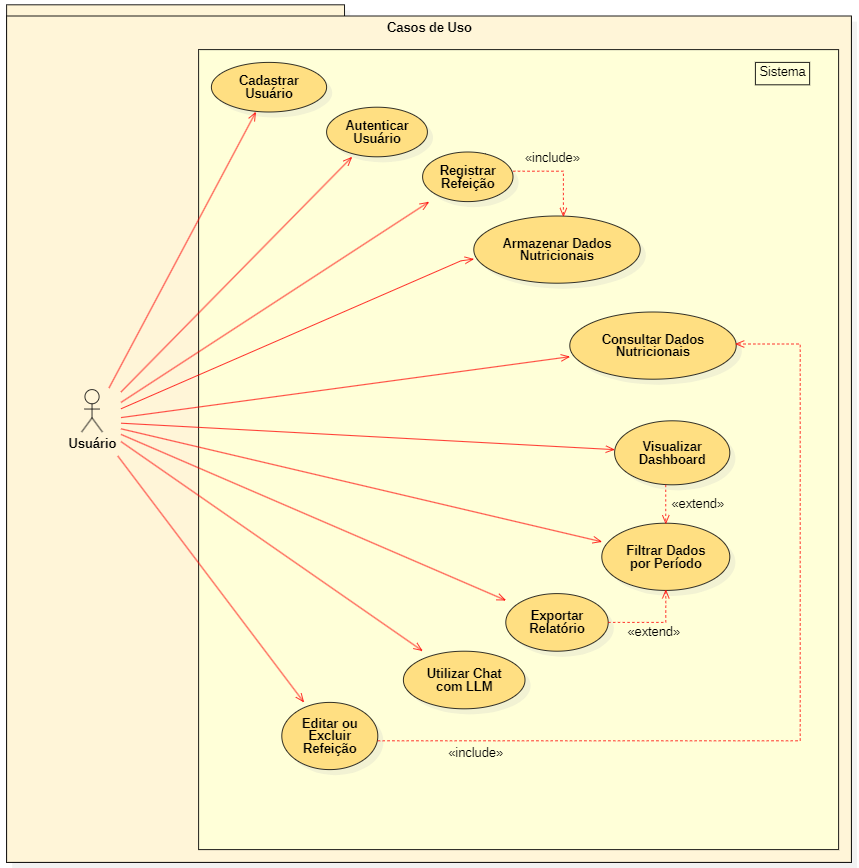
\includegraphics[width=0.92\textwidth]{Figuras/diagrama-casos-uso.png}\\
    \small{\textbf{Fonte}: Autor (2025).}
    \label{fig:diag-casos-uso}
\end{figure}

Na tabela \ref{tab:casos-de-uso} a seguir, estão listados os casos de uso identificados, juntamente com o seu nome. Cada caso de uso representa uma funcionalidade específica do sistema e está associado a um código único para facilitar a referência.

\begin{longtable}[c]{|l|l|}
\caption{Casos de uso e seus códigos.}
\label{tab:casos-de-uso}\\
\hline
\textbf{Código} & \textbf{Descrição}           \\ \hline
\endfirsthead
\endhead
UC01            & Cadastrar Usuário            \\ \hline
UC02            & Autenticar Usuário           \\ \hline
UC03            & Registrar Refeição           \\ \hline
UC04            & Armazenar Dados Nutricionais \\ \hline
UC05            & Consultar Dados Nutricionais \\ \hline
UC06            & Visualizar Dashboard         \\ \hline
UC07            & Filtrar Dados do Período     \\ \hline
UC08            & Exportar Relatório           \\ \hline
UC09            & Utilizar Chat com LLM        \\ \hline
UC10            & Editar ou Excluir Refeição   \\ \hline
\end{longtable}
\begin{center}
    \small{\textbf{Fonte}: Autor (2025).}
\end{center}

Com os casos de uso definidos, o próximo passo é fazer a sua associação com os requisitos funcionais, garantindo que todas as funcionalidades do sistema estejam contempladas. A tabela \ref{tab:casos-uso-requisitos-funcionais} a seguir apresenta essa associação, indicando quais casos de uso atendem a cada requisito funcional.

\begin{table}[h]
    \centering
    \caption{Casos de uso e sua associação com os Requisistos Funcionais.}
    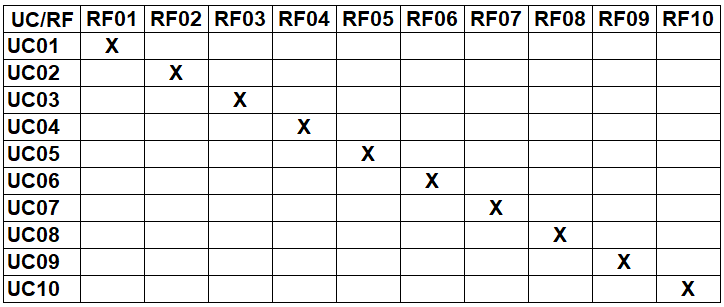
\includegraphics[width=0.92\textwidth]{Tabelas/casos-uso-relacao-reqs-func.png}\\
    \small{\textbf{Fonte}: Autor (2025).}
    \label{tab:casos-uso-requisitos-funcionais}
\end{table}


\section{Definição completa dos Casos de Uso}

A seguir, são apresentados os casos de uso detalhados, com suas descrições, pré-condições, pós-condições e fluxos de eventos. Esses detalhes são essenciais para compreender como cada funcionalidade será implementada e como o usuário interagirá com o sistema.

% UC01 - Cadastrar Usuário
\subsection{UC01 - Cadastrar Usuário}

\begin{longtable}[c]{|p{0.48\textwidth}|p{0.48\textwidth}|}
\caption{UC01: Cadastrar Usuário}
\label{tab:uc01}\\
\hline
\multicolumn{1}{|p{0.48\textwidth}|}{\textbf{Nome}} &
  \begin{tabular}[c]{@{}p{0.48\textwidth}@{}}UC01: Cadastrar Usuário\end{tabular} \\ \hline
\endfirsthead
%
\endhead
%
\multicolumn{1}{|p{0.48\textwidth}|}{\textbf{Atores}} &
  \begin{tabular}[c]{@{}p{0.48\textwidth}@{}}Usuário\end{tabular} \\ \hline
\multicolumn{1}{|p{0.48\textwidth}|}{\textbf{Descrição}} &
  \begin{tabular}[c]{@{}p{0.48\textwidth}@{}}Permite que um novo usuário crie uma conta no sistema informando os dados obrigatórios, garantindo a unicidade do login e a segurança das informações.\end{tabular} \\ \hline
\multicolumn{1}{|p{0.48\textwidth}|}{\textbf{Pré-condições}} &
  \begin{tabular}[c]{@{}p{0.48\textwidth}@{}}O usuário deve ter acessado a aplicação; O usuário não pode estar autenticado; Não deve existir outra conta com o mesmo login.\end{tabular} \\ \hline
\multicolumn{1}{|p{0.48\textwidth}|}{\textbf{Pós-condições}} &
  \begin{tabular}[c]{@{}p{0.48\textwidth}@{}}Conta do usuário criada, pronta para autenticar.\end{tabular} \\ \hline
\multicolumn{2}{|c|}{\textbf{Fluxo Básico}} \\ \hline
\multicolumn{1}{|c|}{\textbf{Ações do Ator}} &
  \multicolumn{1}{c|}{\textbf{Ações do Sistema}} \\ \hline
\multicolumn{1}{|p{0.48\textwidth}|}{\begin{tabular}[c]{@{}p{0.48\textwidth}@{}}1. Acessa a tela de cadastro pelo menu inicial ou por link de criar conta.\end{tabular}} &
   \\ \hline
\multicolumn{1}{|p{0.48\textwidth}|}{} &
  \begin{tabular}[c]{@{}p{0.48\textwidth}@{}}2. Exibe formulário de cadastro com campos obrigatórios (login/e-mail; senha; confirmação da senha; data de nascimento; aceite dos termos).\end{tabular} \\ \hline
\multicolumn{1}{|p{0.48\textwidth}|}{\begin{tabular}[c]{@{}p{0.48\textwidth}@{}}3. Preenche as informações de forma adequada.\end{tabular}} &
   \\ \hline
\multicolumn{1}{|p{0.48\textwidth}|}{\begin{tabular}[c]{@{}p{0.48\textwidth}@{}}4. Clica no botão ``Cadastrar" para submeter as informações digitadas.\end{tabular}} &
   \\ \hline
\multicolumn{1}{|p{0.48\textwidth}|}{} &
  \begin{tabular}[c]{@{}p{0.48\textwidth}@{}}5. Valida se todos os campos obrigatórios foram preenchidos (RN01, RN02, RN08, RN10).\end{tabular} \\ \hline
\multicolumn{1}{|p{0.48\textwidth}|}{} &
  \begin{tabular}[c]{@{}p{0.48\textwidth}@{}}6. Valida o formato do e-mail (RN04).\end{tabular} \\ \hline
\multicolumn{1}{|p{0.48\textwidth}|}{} &
  \begin{tabular}[c]{@{}p{0.48\textwidth}@{}}7. Valida a força da senha (RN05, RN06).\end{tabular} \\ \hline
\multicolumn{1}{|p{0.48\textwidth}|}{} &
  \begin{tabular}[c]{@{}p{0.48\textwidth}@{}}8. Verifica se o login já está cadastrado (RN03).\end{tabular} \\ \hline
\multicolumn{1}{|p{0.48\textwidth}|}{} &
  \begin{tabular}[c]{@{}p{0.48\textwidth}@{}}9. Valida a idade do usuário (RN08).\end{tabular} \\ \hline
\multicolumn{1}{|p{0.48\textwidth}|}{} &
  \begin{tabular}[c]{@{}p{0.48\textwidth}@{}}10. Valida a aceitação dos termos (RN10).\end{tabular} \\ \hline
\multicolumn{1}{|p{0.48\textwidth}|}{} &
  \begin{tabular}[c]{@{}p{0.48\textwidth}@{}}11. Ao aprovar todas as validações, armazena os dados do usuário, criptografa a senha (RN07) e registra a data e hora do cadastro (RN11).\end{tabular} \\ \hline
\multicolumn{1}{|p{0.48\textwidth}|}{} &
  \begin{tabular}[c]{@{}p{0.48\textwidth}@{}}12. Exibe a mensagem de sucesso ``Usuário cadastrado com sucesso!"\end{tabular} \\ \hline
\multicolumn{1}{|p{0.48\textwidth}|}{} &
  \begin{tabular}[c]{@{}p{0.48\textwidth}@{}}13. Redireciona o usuário para a página de login.\end{tabular} \\ \hline
\multicolumn{2}{|c|}{\textbf{Regras de Negócio}} \\ \hline
\multicolumn{1}{|p{0.48\textwidth}|}{RN01} &
  \begin{tabular}[c]{@{}p{0.48\textwidth}@{}}O campo login (e-mail) é obrigatório.\end{tabular} \\ \hline
\multicolumn{1}{|p{0.48\textwidth}|}{RN02} &
  \begin{tabular}[c]{@{}p{0.48\textwidth}@{}}O campo de senha é obrigatório.\end{tabular} \\ \hline
\multicolumn{1}{|p{0.48\textwidth}|}{RN03} &
  \begin{tabular}[c]{@{}p{0.48\textwidth}@{}}O login deve ser único no sistema.\end{tabular} \\ \hline
\multicolumn{1}{|p{0.48\textwidth}|}{RN04} &
  \begin{tabular}[c]{@{}p{0.48\textwidth}@{}}O email deve estar em formato válido.\end{tabular} \\ \hline
\multicolumn{1}{|p{0.48\textwidth}|}{RN05} &
  \begin{tabular}[c]{@{}p{0.48\textwidth}@{}}A senha deve ter no mínimo 8 caracteres.\end{tabular} \\ \hline
\multicolumn{1}{|p{0.48\textwidth}|}{RN06} &
  \begin{tabular}[c]{@{}p{0.48\textwidth}@{}}A senha deve conter pelo menos uma letra maiúscula, uma minúscula, um número e um caractere especial.\end{tabular} \\ \hline
\multicolumn{1}{|p{0.48\textwidth}|}{RN07} &
  \begin{tabular}[c]{@{}p{0.48\textwidth}@{}}O sistema deve armazenar a senha de forma criptografada.\end{tabular} \\ \hline
\multicolumn{1}{|p{0.48\textwidth}|}{RN08} &
  \begin{tabular}[c]{@{}p{0.48\textwidth}@{}}O cadastro só é permitido para maiores de 18 anos.\end{tabular} \\ \hline
\multicolumn{1}{|p{0.48\textwidth}|}{RN09} &
  \begin{tabular}[c]{@{}p{0.48\textwidth}@{}}O sistema deve validar a regra de negócio RNF02 (autenticação via JWT).\end{tabular} \\ \hline
\multicolumn{1}{|p{0.48\textwidth}|}{RN10} &
  \begin{tabular}[c]{@{}p{0.48\textwidth}@{}}O usuário deve aceitar os termos de uso e política de privacidade.\end{tabular} \\ \hline
\multicolumn{1}{|p{0.48\textwidth}|}{RN11} &
  \begin{tabular}[c]{@{}p{0.48\textwidth}@{}}O sistema deve registrar a data e hora do cadastro.\end{tabular} \\ \hline
\multicolumn{2}{|c|}{\textbf{Fluxo Alternativo A: login já cadastrado}} \\ \hline
\multicolumn{1}{|c|}{\textbf{Ações do Ator}} &
  \multicolumn{1}{c|}{\textbf{Ações do Sistema}} \\ \hline
\multicolumn{1}{|p{0.48\textwidth}|}{\begin{tabular}[c]{@{}p{0.48\textwidth}@{}}1. Preenche o formulário com um e-mail já existente clica em ``Cadastrar".\end{tabular}} &
   \\ \hline
\multicolumn{1}{|p{0.48\textwidth}|}{} &
  \begin{tabular}[c]{@{}p{0.48\textwidth}@{}}2. Valida unicidade do login e identifica duplicidade.\end{tabular} \\ \hline
\multicolumn{1}{|p{0.48\textwidth}|}{} &
  \begin{tabular}[c]{@{}p{0.48\textwidth}@{}}3. Exibe mensagem de erro ``E-mail já cadastrado. Tente outro e-mail."\end{tabular} \\ \hline
\multicolumn{2}{|c|}{\textbf{Fluxo Alternativo B: senha fraca ou inválida}} \\ \hline
\multicolumn{1}{|c|}{\textbf{Ações do Ator}} &
  \multicolumn{1}{c|}{\textbf{Ações do Sistema}} \\ \hline
\multicolumn{1}{|p{0.48\textwidth}|}{\begin{tabular}[c]{@{}p{0.48\textwidth}@{}}1. Preenche o campo de senha com valor que não atende aos critérios e clica em ``Cadastrar".\end{tabular}} &
   \\ \hline
\multicolumn{1}{|p{0.48\textwidth}|}{} &
  \begin{tabular}[c]{@{}p{0.48\textwidth}@{}}2. Valida a força da senha e identifica não conformidade.\end{tabular} \\ \hline
\multicolumn{1}{|p{0.48\textwidth}|}{} &
  \begin{tabular}[c]{@{}p{0.48\textwidth}@{}}3. Exibe mensagem de erro detalhando os requisitos mínimos da senha\end{tabular} \\ \hline
\multicolumn{2}{|c|}{\textbf{Fluxo Alternativo C: campos obrigatórios não preenchidos}} \\ \hline
\multicolumn{1}{|c|}{\textbf{Ações do Ator}} &
  \multicolumn{1}{c|}{\textbf{Ações do Sistema}} \\ \hline
\multicolumn{1}{|p{0.48\textwidth}|}{\begin{tabular}[c]{@{}p{0.48\textwidth}@{}}1. Deixa um ou mais campos obrigatórios em branco e clica em ``Cadastrar".\end{tabular}} &
   \\ \hline
\multicolumn{1}{|p{0.48\textwidth}|}{} &
  \begin{tabular}[c]{@{}p{0.48\textwidth}@{}}2. Valida preenchimento dos campos e identifica ausência.\end{tabular} \\ \hline
\multicolumn{1}{|p{0.48\textwidth}|}{} &
  \begin{tabular}[c]{@{}p{0.48\textwidth}@{}}3. Exibe mensagem de erro informando quais campos precisam ser preenchidos.\end{tabular} \\ \hline
\multicolumn{2}{|c|}{\textbf{Fluxo Alternativo D: usuário menor de 18 anos}} \\ \hline
\multicolumn{1}{|c|}{\textbf{Ações do Ator}} &
  \multicolumn{1}{c|}{\textbf{Ações do Sistema}} \\ \hline
\multicolumn{1}{|p{0.48\textwidth}|}{\begin{tabular}[c]{@{}p{0.48\textwidth}@{}}1. Informa data de nascimento que indica idade inferior a 18 anos e clica em “Cadastrar”.\end{tabular}} &
   \\ \hline
\multicolumn{1}{|p{0.48\textwidth}|}{} &
  \begin{tabular}[c]{@{}p{0.48\textwidth}@{}}2. Valida idade e identifica restrição.\end{tabular} \\ \hline
\multicolumn{1}{|p{0.48\textwidth}|}{} &
  \begin{tabular}[c]{@{}p{0.48\textwidth}@{}}3. Exibe mensagem de erro ``Cadastro permitido apenas para maiores de 18 anos."\end{tabular} \\ \hline
\multicolumn{2}{|c|}{\textbf{Fluxo Alternativo E: e-mail em formato inválido}} \\ \hline
\multicolumn{1}{|c|}{\textbf{Ações do Ator}} &
  \multicolumn{1}{c|}{\textbf{Ações do Sistema}} \\ \hline
\multicolumn{1}{|p{0.48\textwidth}|}{\begin{tabular}[c]{@{}p{0.48\textwidth}@{}}1. Preenche o campo de e-mail com formato incorreto e clica em ``Cadastrar".\end{tabular}} &
   \\ \hline
\multicolumn{1}{|p{0.48\textwidth}|}{} &
  \begin{tabular}[c]{@{}p{0.48\textwidth}@{}}2. Valida formato do e-mail e identifica erro.\end{tabular} \\ \hline
\multicolumn{1}{|p{0.48\textwidth}|}{} &
  \begin{tabular}[c]{@{}p{0.48\textwidth}@{}}3. Exibe mensagem de erro ``E-mail em formato inválido."\end{tabular} \\ \hline
\multicolumn{2}{|c|}{\textbf{Fluxo Alternativo F: recarregamento da página}} \\ \hline
\multicolumn{1}{|c|}{\textbf{Ações do Ator}} &
  \multicolumn{1}{c|}{\textbf{Ações do Sistema}} \\ \hline
\multicolumn{1}{|p{0.48\textwidth}|}{\begin{tabular}[c]{@{}p{0.48\textwidth}@{}}1. Durante o preenchimento do formulário, recarrega a página do navegador.\end{tabular}} &
   \\ \hline
\multicolumn{1}{|p{0.48\textwidth}|}{} &
  \begin{tabular}[c]{@{}p{0.48\textwidth}@{}}2. Recarrega a tela de cadastro, perdendo todos os dados não salvos.\end{tabular} \\ \hline
\end{longtable}

% UC02 - Autenticar Usuário
\subsection{UC02 - Autenticar Usuário}

\begin{longtable}[c]{|p{0.48\textwidth}|p{0.48\textwidth}|}
\caption{UC02: Autenticar Usuário}
\label{tab:uc02}\\
\hline
\multicolumn{1}{|p{0.48\textwidth}|}{\textbf{Nome}} &
  \begin{tabular}[c]{@{}p{0.48\textwidth}@{}}UC02: Autenticar Usuário\end{tabular} \\ \hline
\endfirsthead
%
\endhead
%
\multicolumn{1}{|p{0.48\textwidth}|}{\textbf{Atores}} &
  \begin{tabular}[c]{@{}p{0.48\textwidth}@{}}Usuário\end{tabular} \\ \hline
\multicolumn{1}{|p{0.48\textwidth}|}{\textbf{Descrição}} &
  \begin{tabular}[c]{@{}p{0.48\textwidth}@{}}Permite que um usuário cadastrado acesse o sistema informando suas credenciais válidas, garantindo a segurança e a privacidade das informações.\end{tabular} \\ \hline
\multicolumn{1}{|p{0.48\textwidth}|}{\textbf{Pré-condições}} &
  \begin{tabular}[c]{@{}p{0.48\textwidth}@{}}O usuário deve ter cadastro prévio no sistema; O usuário não pode estar autenticado.\end{tabular} \\ \hline
\multicolumn{1}{|p{0.48\textwidth}|}{\textbf{Pós-condições}} &
  \begin{tabular}[c]{@{}p{0.48\textwidth}@{}}Usuário autenticado, sessão iniciada.\end{tabular} \\ \hline
\multicolumn{2}{|c|}{\textbf{Fluxo Básico}} \\ \hline
\multicolumn{1}{|c|}{\textbf{Ações do Ator}} &
  \multicolumn{1}{c|}{\textbf{Ações do Sistema}} \\ \hline
\multicolumn{1}{|p{0.48\textwidth}|}{\begin{tabular}[c]{@{}p{0.48\textwidth}@{}}1. Acessa a tela de login pelo menu inicial.\end{tabular}} &
   \\ \hline
\multicolumn{1}{|p{0.48\textwidth}|}{} &
  \begin{tabular}[c]{@{}p{0.48\textwidth}@{}}2. Exibe formulário de autenticação com campos obrigatórios (login/e-mail e senha).\end{tabular} \\ \hline
\multicolumn{1}{|p{0.48\textwidth}|}{\begin{tabular}[c]{@{}p{0.48\textwidth}@{}}3. Preenche o campo de e-mail e senha.\end{tabular}} &
   \\ \hline
\multicolumn{1}{|p{0.48\textwidth}|}{\begin{tabular}[c]{@{}p{0.48\textwidth}@{}}4. Clica no botão ``Entrar'' para submeter as informações.\end{tabular}} &
   \\ \hline
\multicolumn{1}{|p{0.48\textwidth}|}{} &
  \begin{tabular}[c]{@{}p{0.48\textwidth}@{}}5. Valida se os campos obrigatórios foram preenchidos (RN01, RN02).\end{tabular} \\ \hline
\multicolumn{1}{|p{0.48\textwidth}|}{} &
  \begin{tabular}[c]{@{}p{0.48\textwidth}@{}}6. Valida o formato do e-mail (RN04).\end{tabular} \\ \hline
\multicolumn{1}{|p{0.48\textwidth}|}{} &
  \begin{tabular}[c]{@{}p{0.48\textwidth}@{}}7. Verifica se existe usuário cadastrado com o e-mail informado (RN12).\end{tabular} \\ \hline
\multicolumn{1}{|p{0.48\textwidth}|}{} &
  \begin{tabular}[c]{@{}p{0.48\textwidth}@{}}8. Valida a senha informada comparando com a senha armazenada (RN13).\end{tabular} \\ \hline
\multicolumn{1}{|p{0.48\textwidth}|}{} &
  \begin{tabular}[c]{@{}p{0.48\textwidth}@{}}9. Gera token de autenticação JWT para o usuário (RN09).\end{tabular} \\ \hline
\multicolumn{1}{|p{0.48\textwidth}|}{} &
  \begin{tabular}[c]{@{}p{0.48\textwidth}@{}}10. Inicia a sessão do usuário autenticado.\end{tabular} \\ \hline
\multicolumn{1}{|p{0.48\textwidth}|}{} &
  \begin{tabular}[c]{@{}p{0.48\textwidth}@{}}11. Redireciona o usuário para a página inicial do sistema.\end{tabular} \\ \hline
\multicolumn{2}{|c|}{\textbf{Regras de Negócio}} \\ \hline
\multicolumn{1}{|p{0.48\textwidth}|}{RN01} &
  \begin{tabular}[c]{@{}p{0.48\textwidth}@{}}O campo login (e-mail) é obrigatório.\end{tabular} \\ \hline
\multicolumn{1}{|p{0.48\textwidth}|}{RN02} &
  \begin{tabular}[c]{@{}p{0.48\textwidth}@{}}O campo de senha é obrigatório.\end{tabular} \\ \hline
\multicolumn{1}{|p{0.48\textwidth}|}{RN04} &
  \begin{tabular}[c]{@{}p{0.48\textwidth}@{}}O email deve estar em formato válido.\end{tabular} \\ \hline
\multicolumn{1}{|p{0.48\textwidth}|}{RN12} &
  \begin{tabular}[c]{@{}p{0.48\textwidth}@{}}O login deve existir no sistema.\end{tabular} \\ \hline
\multicolumn{1}{|p{0.48\textwidth}|}{RN13} &
  \begin{tabular}[c]{@{}p{0.48\textwidth}@{}}A senha informada deve ser igual à senha cadastrada.\end{tabular} \\ \hline
\multicolumn{1}{|p{0.48\textwidth}|}{RN09} &
  \begin{tabular}[c]{@{}p{0.48\textwidth}@{}}O sistema deve autenticar o usuário via JWT.\end{tabular} \\ \hline
\multicolumn{2}{|c|}{\textbf{Fluxo Alternativo A: login inexistente}} \\ \hline
\multicolumn{1}{|c|}{\textbf{Ações do Ator}} &
  \multicolumn{1}{c|}{\textbf{Ações do Sistema}} \\ \hline
\multicolumn{1}{|p{0.48\textwidth}|}{\begin{tabular}[c]{@{}p{0.48\textwidth}@{}}1. Preenche o campo de e-mail com um login não cadastrado e clica em ``Entrar''.\end{tabular}} &
   \\ \hline
\multicolumn{1}{|p{0.48\textwidth}|}{} &
  \begin{tabular}[c]{@{}p{0.48\textwidth}@{}}2. Verifica inexistência do login informado.\end{tabular} \\ \hline
\multicolumn{1}{|p{0.48\textwidth}|}{} &
  \begin{tabular}[c]{@{}p{0.48\textwidth}@{}}3. Exibe mensagem de erro ``Usuário não encontrado.''\end{tabular} \\ \hline
\multicolumn{2}{|c|}{\textbf{Fluxo Alternativo B: senha incorreta}} \\ \hline
\multicolumn{1}{|c|}{\textbf{Ações do Ator}} &
  \multicolumn{1}{c|}{\textbf{Ações do Sistema}} \\ \hline
\multicolumn{1}{|p{0.48\textwidth}|}{\begin{tabular}[c]{@{}p{0.48\textwidth}@{}}1. Preenche o campo de senha com valor incorreto e clica em ``Entrar''.\end{tabular}} &
   \\ \hline
\multicolumn{1}{|p{0.48\textwidth}|}{} &
  \begin{tabular}[c]{@{}p{0.48\textwidth}@{}}2. Valida a senha e identifica divergência.\end{tabular} \\ \hline
\multicolumn{1}{|p{0.48\textwidth}|}{} &
  \begin{tabular}[c]{@{}p{0.48\textwidth}@{}}3. Exibe mensagem de erro ``Senha incorreta.''\end{tabular} \\ \hline
\multicolumn{2}{|c|}{\textbf{Fluxo Alternativo C: campos obrigatórios não preenchidos}} \\ \hline
\multicolumn{1}{|c|}{\textbf{Ações do Ator}} &
  \multicolumn{1}{c|}{\textbf{Ações do Sistema}} \\ \hline
\multicolumn{1}{|p{0.48\textwidth}|}{\begin{tabular}[c]{@{}p{0.48\textwidth}@{}}1. Deixa o campo de e-mail e/ou senha em branco e clica em ``Entrar''.\end{tabular}} &
   \\ \hline
\multicolumn{1}{|p{0.48\textwidth}|}{} &
  \begin{tabular}[c]{@{}p{0.48\textwidth}@{}}2. Valida preenchimento dos campos e identifica ausência.\end{tabular} \\ \hline
\multicolumn{1}{|p{0.48\textwidth}|}{} &
  \begin{tabular}[c]{@{}p{0.48\textwidth}@{}}3. Exibe mensagem de erro informando que todos os campos são obrigatórios.\end{tabular} \\ \hline
\multicolumn{2}{|c|}{\textbf{Fluxo Alternativo D: e-mail em formato inválido}} \\ \hline
\multicolumn{1}{|c|}{\textbf{Ações do Ator}} &
  \multicolumn{1}{c|}{\textbf{Ações do Sistema}} \\ \hline
\multicolumn{1}{|p{0.48\textwidth}|}{\begin{tabular}[c]{@{}p{0.48\textwidth}@{}}1. Preenche o campo de e-mail com formato inválido e clica em ``Entrar''.\end{tabular}} &
   \\ \hline
\multicolumn{1}{|p{0.48\textwidth}|}{} &
  \begin{tabular}[c]{@{}p{0.48\textwidth}@{}}2. Valida formato do e-mail e identifica erro.\end{tabular} \\ \hline
\multicolumn{1}{|p{0.48\textwidth}|}{} &
  \begin{tabular}[c]{@{}p{0.48\textwidth}@{}}3. Exibe mensagem de erro ``E-mail em formato inválido.''\end{tabular} \\ \hline
\multicolumn{2}{|c|}{\textbf{Fluxo Alternativo E: recarregamento da página}} \\ \hline
\multicolumn{1}{|c|}{\textbf{Ações do Ator}} &
  \multicolumn{1}{c|}{\textbf{Ações do Sistema}} \\ \hline
\multicolumn{1}{|p{0.48\textwidth}|}{\begin{tabular}[c]{@{}p{0.48\textwidth}@{}}1. Durante o preenchimento do formulário, recarrega a página do navegador.\end{tabular}} &
   \\ \hline
\multicolumn{1}{|p{0.48\textwidth}|}{} &
  \begin{tabular}[c]{@{}p{0.48\textwidth}@{}}2. Recarrega a tela de login, perdendo todos os dados não salvos.\end{tabular} \\ \hline
\end{longtable}

\subsection{UC03 - Registrar Refeição}   %Experimentos e resultados
\chapter{Rastreamento de Requisitos}\label{cap:5-rast-req}

   %Conclusoes e trabalhos futuros
\chapter{Verificação e Validação de Requisitos}\label{cap:6-verif-valid-req}

A verificação e validação de requisitos são etapas fundamentais para garantir a qualidade, a clareza e a aderência dos requisitos às necessidades dos stakeholders e às restrições do projeto. Enquanto a verificação busca responder à pergunta ``O sistema está sendo construído corretamente?'', a validação busca garantir que ``O sistema que está sendo construído é o desejado pelos clientes e usuários?''. Ambas as atividades são essenciais para evitar retrabalho, ambiguidades e falhas no desenvolvimento do sistema.

\section{Matriz de Verificação dos Requisitos Funcionais}

A verificação dos requisitos funcionais foi realizada com base nos nove problemas clássicos apresentados em aula: validade, consistência, completeza, realismo, facilidade de verificação (compreensibilidade), ambiguidade, facilidade de rastreamento, redundância e conformidade. O tempo total gasto na análise foi de 18 minutos.

\begin{longtable}{|p{0.14\textwidth}|*{10}{>{\centering\arraybackslash}p{0.057\textwidth}|}}
\caption{Matriz de Verificação dos Requisitos Funcionais. \textbf{Legenda:} X = apresenta o problema; célula em branco = não apresenta o problema.}
\label{tab:verificacao-reqs-funcionais}\\
\hline
\textbf{Ponto de Verificação} & \textbf{RF01} & \textbf{RF02} & \textbf{RF03} & \textbf{RF04} & \textbf{RF05} & \textbf{RF06} & \textbf{RF07} & \textbf{RF08} & \textbf{RF09} & \textbf{RF10} \\
\hline
\endfirsthead
\endhead
Validade &  &  &  &  &  &  &  &  &  &  \\
\hline
Consistência &  &  &  &  &  &  &  &  &  &  \\
\hline
Completeza &  &  & X &  &  & X & X &  &  &  \\
\hline
Realismo &  &  &  & X &  & X &  & X &  &  \\
\hline
Verificação &  &  &  &  &  &  &  &  &  &  \\
\hline
Ambiguidade &  &  & X &  &  & X & X &  &  &  \\
\hline
Rastreamento &  &  &  &  &  &  &  &  &  &  \\
\hline
Redundância &  &  &  &  &  &  &  &  &  &  \\
\hline
Conformidade &  &  &  &  &  &  &  &  &  &  \\
\hline
\end{longtable}

\section{Matriz de Verificação dos Requisitos Não Funcionais}

A verificação dos requisitos não funcionais também foi realizada com base nos mesmos nove problemas. O tempo total gasto na análise foi de 15 minutos.

\begin{longtable}{|p{0.14\textwidth}|*{10}{>{\centering\arraybackslash}p{0.057\textwidth}|}}
\caption{Matriz de Verificação dos Requisitos Não Funcionais. \textbf{Legenda:} X = apresenta o problema; célula em branco = não apresenta o problema.}
\label{tab:verificacao-reqs-naofuncionais}\\
\hline
\textbf{Ponto de Verificação} & \textbf{RNF 01} & \textbf{RNF 02} & \textbf{RNF 03} & \textbf{RNF 04} & \textbf{RNF 05} & \textbf{RNF 06} & \textbf{RNF 07} & \textbf{RNF 08} & \textbf{RNF 09} & \textbf{RNF 10} \\
\hline
\endfirsthead
\endhead
Validade &  &  &  &  &  &  &  &  &  &  \\
\hline
Consistência &  &  &  &  &  &  &  &  &  &  \\
\hline
Completeza &  &  &  &  & X &  &  &  &  & X \\
\hline
Realismo &  &  &  &  &  &  & X &  &  & X \\
\hline
Verificação &  &  &  &  & X &  &  &  &  &  \\
\hline
Ambiguidade &  &  &  &  & X & X &  &  &  &  \\
\hline
Rastreamento &  &  &  &  &  &  &  &  &  &  \\
\hline
Redundância &  &  &  &  &  &  &  &  &  &  \\
\hline
Conformidade &  &  &  &  &  &  &  &  &  &  \\
\hline
\end{longtable}

\section{Ações para Resolução dos Problemas Identificados}

A partir das matrizes de verificação, foram identificados alguns requisitos que apresentam problemas de completeza, ambiguidade, realismo ou verificabilidade. As principais ações propostas para resolução ou mitigação desses problemas são:

\begin{itemize}
    \item \textbf{RF03, RF06, RF07, RNF05, RNF06, RNF10}: Refinar as descrições para detalhar critérios objetivos, remover termos vagos e garantir que todos os aspectos esperados estejam descritos.
    \item \textbf{RF04, RF08, RNF07, RNF10}: Consultar a equipe técnica para garantir que a integração, tempo de resposta e capacidade são factíveis.
    \item \textbf{RNF05}: Especificar critérios mensuráveis para acessibilidade (ex: conformidade com WCAG AA).
    \item \textbf{RNF05, RF06, RF07, RNF06}: Especificar termos e métricas claras para eliminar ambiguidade.
\end{itemize}

\section{Casos de Teste para os Requisitos Funcionais}

A seguir, são apresentados casos de teste para cada um dos 10 requisitos funcionais, seguindo a estrutura recomendada:

\begin{longtable}{|p{0.06\textwidth}|p{0.20\textwidth}|p{0.15\textwidth}|p{0.12\textwidth}|p{0.15\textwidth}|p{0.12\textwidth}|}
\caption{Casos de Teste para os Requisitos Funcionais}
\label{tab:casos-teste-reqs-funcionais}\\
\hline
\textbf{Req.} & \textbf{Descrição} & \textbf{Pré-condição} & \textbf{Entrada} & \textbf{Procedimento} & \textbf{Resultado Esperado} \\
\hline
\endfirsthead
\endhead
RF01 & Cadastro de usuário com e-mail e senha & Usuário não cadastrado & E-mail válido, senha válida & Preencher formulário e submeter & Usuário cadastrado com sucesso \\
\hline
RF02 & Autenticação de usuário (login/logout) & Usuário cadastrado & E-mail e senha corretos & Preencher login e submeter & Usuário autenticado e sessão iniciada \\
\hline
RF03 & Registro de refeições (descrição livre ou por ingredientes) & Usuário autenticado & Descrição da refeição, ingredientes & Preencher e submeter registro & Refeição registrada e associada ao usuário \\
\hline
RF04 & Consulta automática de dados nutricionais via LLM & Refeição registrada & Seleção de refeição & Solicitar consulta nutricional & Dados nutricionais exibidos \\
\hline
RF05 & Armazenamento de dados nutricionais (kcal, macros, micros) & Dados nutricionais disponíveis & Dados nutricionais & Armazenar dados & Dados salvos e disponíveis para consulta \\
\hline
RF06 & Dashboard com gráficos de consumo (período personalizável) & Dados nutricionais registrados & Seleção de período & Acessar dashboard & Gráficos exibidos corretamente \\
\hline
RF07 & Filtros temporais para análise (dia/semana/mês) & Dados registrados & Seleção de filtro (dia/semana/mês) & Aplicar filtro & Dados filtrados exibidos \\
\hline
RF08 & Chat integrado para consultar LLM & Usuário autenticado & Pergunta enviada ao chat & Enviar mensagem & Resposta do LLM exibida \\
\hline
RF09 & Exportação de relatórios em PDF/CSV & Dados disponíveis & Seleção de formato & Solicitar exportação & Arquivo gerado e disponível para download \\
\hline
RF10 & Edição/exclusão de refeições registradas & Refeição registrada & Seleção de refeição, nova informação ou comando de exclusão & Editar ou excluir refeição & Alteração ou exclusão realizada com sucesso \\
\hline
\end{longtable}

\textbf{Fonte}: Elaborado pelo autor (2025).

\section{Requisitos Refinados e Corrigidos}

Com base nas ações corretivas propostas e na análise detalhada das matrizes de verificação, todos os requisitos funcionais e não funcionais foram revisados e aprimorados para garantir clareza, objetividade, mensurabilidade e aderência às melhores práticas de engenharia de requisitos. A seguir, apresentam-se os requisitos refinados, já com as correções implementadas, mantendo a coesão e o alinhamento com os capítulos anteriores.

\subsection{Requisitos Funcionais Refinados}

\begin{longtable}{|l|p{0.70\textwidth}|}
\caption{Requisitos Funcionais Refinados}
\label{tab:reqs-funcionais-refinados}\\
\hline
\textbf{Código} & \textbf{Descrição Refinada} \\
\hline
\endfirsthead
\endhead
RF01 & O sistema deve permitir o cadastro de novos usuários mediante preenchimento de e-mail válido e senha que atenda aos critérios de segurança definidos (mínimo 8 caracteres, incluindo letra maiúscula, minúscula, número e caractere especial), garantindo unicidade do e-mail e confirmação do aceite dos termos de uso. \\
\hline
RF02 & O sistema deve autenticar usuários cadastrados por meio de login com e-mail e senha, utilizando autenticação JWT com refresh tokens, permitindo início e término de sessão de forma segura. \\
\hline
RF03 & O sistema deve possibilitar o registro de refeições, permitindo ao usuário inserir uma descrição livre ou selecionar ingredientes de uma lista padronizada, associando cada refeição ao usuário autenticado e armazenando data e hora do registro. \\
\hline
RF04 & O sistema deve consultar automaticamente, via integração com LLM, os dados nutricionais das refeições registradas, apresentando informações detalhadas de calorias, macronutrientes e micronutrientes em até 30 segundos após a solicitação. \\
\hline
RF05 & O sistema deve armazenar de forma estruturada os dados nutricionais (kcal, macronutrientes e micronutrientes) de cada refeição registrada, garantindo backup diário e criptografia dos dados sensíveis. \\
\hline
RF06 & O sistema deve disponibilizar um dashboard interativo com gráficos de consumo nutricional, permitindo ao usuário personalizar o período de análise (dia, semana, mês), com renderização dos gráficos em até 5 segundos e precisão mínima de 99,9\%. \\
\hline
RF07 & O sistema deve oferecer filtros temporais (dia, semana, mês) para análise dos dados nutricionais, assegurando que os resultados exibidos correspondam exatamente ao período selecionado pelo usuário. \\
\hline
RF08 & O sistema deve disponibilizar um chat integrado para que o usuário possa enviar perguntas ao LLM, recebendo respostas em linguagem natural em até 30 segundos, com registro do histórico de interações. \\
\hline
RF09 & O sistema deve permitir a exportação de relatórios nutricionais em formato PDF e CSV, contendo todos os dados registrados pelo usuário no período selecionado, com geração do arquivo em até 10 segundos e suporte a até 10.000 registros por mês por usuário. \\
\hline
RF10 & O sistema deve permitir a edição e exclusão de refeições previamente registradas pelo usuário, garantindo atualização imediata dos dados nutricionais e manutenção do histórico de alterações. \\
\hline
\end{longtable}

\subsection{Requisitos Não Funcionais Refinados}

\begin{longtable}{|l|p{0.70\textwidth}|}
\caption{Requisitos Não Funcionais Refinados}
\label{tab:reqs-naofuncionais-refinados}\\
\hline
\textbf{Código} & \textbf{Descrição Refinada} \\
\hline
\endfirsthead
\endhead
RNF01 & O tempo de resposta para consultas ao LLM deve ser inferior a 30 segundos em 99,9\% das solicitações. \\
\hline
RNF02 & O sistema deve utilizar autenticação baseada em JWT com refresh tokens, protegendo todas as rotas sensíveis e garantindo renovação segura de sessão. \\
\hline
RNF03 & O sistema deve realizar backup automático diário de todos os dados nutricionais dos usuários, com retenção mínima de 30 dias e possibilidade de restauração completa. \\
\hline
RNF04 & Os gráficos do dashboard devem ser renderizados em até 5 segundos após a solicitação do usuário, independentemente do volume de dados. \\
\hline
RNF05 & A interface do sistema deve ser acessível, atendendo integralmente ao padrão WCAG 2.1 nível AA, incluindo navegação por teclado, contraste adequado e textos alternativos em imagens. \\
\hline
RNF06 & Os dados analíticos apresentados devem possuir precisão mínima de 99,9\%, com validação automática de consistência a cada atualização de dados. \\
\hline
RNF07 & A integração com o serviço Ollama (LLM) deve apresentar disponibilidade mínima de 99,95\% ao mês, com monitoramento contínuo e alertas automáticos em caso de falha. \\
\hline
RNF08 & Todos os dados sensíveis armazenados devem ser protegidos por criptografia AES-256, incluindo dados pessoais e nutricionais. \\
\hline
RNF09 & O processamento de consultas ao LLM deve ser assíncrono, permitindo múltiplas solicitações simultâneas sem bloqueio da interface do usuário. \\
\hline
RNF10 & O sistema deve suportar, no mínimo, 10.000 registros de refeições por mês para cada usuário, sem degradação perceptível de desempenho. \\
\hline
\end{longtable}

\begin{center}
    \small{\textbf{Fonte}: Elaborado pelo autor (2025).}
\end{center}
   




\chapter{Gerência de Requisitos com Rastreamento de Dependências}\label{cap:7-ger-req-rast-dep}

   




\chapter{Gerenciamento de Requisitos com Use Case Points}\label{cap:8-ger-req-use-case-points}

   
\chapter{Prioridade de Requisitos com Use Case Points}\label{cap:9-prio-req}

A priorização de requisitos é uma etapa fundamental para alinhar o desenvolvimento do sistema às necessidades dos stakeholders e otimizar o uso de recursos. Segundo a abordagem apresentada em aula, a classificação dos requisitos pode ser feita em três níveis: Essencial (crítico), Importante e Desejável (útil). A priorização facilita o diálogo entre usuários e equipe de desenvolvimento, permitindo identificar o conjunto mínimo de funcionalidades necessárias para atender aos objetivos do projeto.

Neste capítulo, será realizada uma análise de redução de escopo baseada na técnica de Use Case Points (UCP) calculada no capítulo anterior, visando uma diminuição de pelo menos 30\% no custo estimado do projeto. Para isso, serão removidos, primeiramente, os casos de uso de menor prioridade (desejáveis), seguidos dos importantes, até atingir a meta de redução.

\section{Redução de 30\% no Custo do Projeto}

O valor total estimado para o projeto, conforme o cálculo dos Use Case Points no capítulo 8, foi de:

\begin{itemize}
    \item \textbf{UCP total:} 52
    \item \textbf{Horas estimadas:} 520
\end{itemize}

Reduzindo em 30\%:

\begin{itemize}
    \item \textbf{UCP reduzido:} 52 $\times$ 0,7 = \textbf{36,4}
    \item \textbf{Horas reduzidas:} 520 $\times$ 0,7 = \textbf{364}
\end{itemize}

Sabendo que o UCP deve ser reduzido para, pelo menos, $36,4$, o próximo passo é identificar quais casos de uso podem ser removidos para atingir essa meta. Portanto, trabalharemos com a redução do valor do UUCP que, de acordo com o capítulo \ref{cap:8-ger-req-use-case-points} é de 93. Neste caso, abaixo consta o cálculo que demonstra a redução necessária:

Cálculo do valor mínimo de UUCP para atingir pelo menos $UCP = 36,4$:
\begin{align*}
    UUCP \times TCF \times ECF &= UCP\\
    UUCP &= \frac{UCP}{TCF \times ECF}\\
    &= \frac{36,4}{1,055 \times 0,53}\\
    &= 65,1
\end{align*}

Portanto, o valor mínimo de UUCP necessário para atingir a meta de redução é de 65,1. Considerando que o UUCP original é 93, a redução necessária é:
\begin{align*}
    UUCP_{Reduzir} &= UUCP - UUCP_{min}\\
    &= 93 - 65,1\\
    &= 27,9
\end{align*}

\section{Seleção dos Casos de Uso Necessários e Suficientes}

Para atingir a meta de redução de pelo menos 30\% no custo do projeto, é necessário que o valor do UUCP (soma dos pontos dos atores e dos casos de uso) seja inferior a 65,1, conforme demonstrado anteriormente. O UUCP original do sistema é 93, composto por UAW = 8 (atores) e UUCW = 85 (casos de uso). Assim, a redução mínima necessária é de 27,9 pontos no UUCP, o que implica a remoção de casos de uso de menor prioridade até que o novo UUCP seja igual ou inferior a 65,1.

A estratégia adotada consiste em remover, primeiramente, os casos de uso classificados como desejáveis, seguidos dos importantes de menor impacto, sempre preservando as funcionalidades essenciais para o funcionamento do sistema.

\subsection{Classificação dos Casos de Uso por Prioridade}

Com base nos requisitos funcionais refinados (capítulo 6), a classificação dos casos de uso é:

\begin{itemize}
    \item \textbf{Essenciais:} RF01 (Cadastro de usuário), RF03 (Registro de refeições), RF04 (Consulta nutricional via LLM), RF05 (Armazenamento de dados nutricionais)
    \item \textbf{Importantes:} RF02 (Autenticação), RF06 (Dashboard), RF08 (Chat LLM), RF10 (Edição/exclusão de refeições)
    \item \textbf{Desejáveis:} RF07 (Filtros temporais), RF09 (Exportação de relatórios)
\end{itemize}

\subsection{Remoção dos Casos de Uso de Menor Prioridade}

A distribuição dos pontos dos casos de uso (UUCW) é:

\begin{itemize}
    \item \textbf{Simples (5 pontos):} RF01, RF02, RF07, RF09, RF10
    \item \textbf{Médio (10 pontos):} RF03, RF05, RF08
    \item \textbf{Complexo (15 pontos):} RF04, RF06
\end{itemize}

O UAW permanece constante em 8, pois não há alteração nos atores do sistema. Portanto, a redução será realizada exclusivamente sobre o UUCW.

% Remoção dos casos de uso de menor prioridade
Removendo inicialmente os casos de uso desejáveis (RF07 e RF09):

\begin{itemize}
    \item Pontos removidos: 5 (RF07) + 5 (RF09) + 1 (ator simples do serviço de exportação de relatórios) = 11
    \item UUCW restante: 85 - 10 = 75
    \item UAW restante: 8 - 1 = 7
    \item UUCP restante: 7 + 75 = 82
\end{itemize}

Ainda não atingiu a meta. Removendo o caso de uso importante de menor impacto (RF10):

\begin{itemize}
    \item Pontos removidos: 5 (RF10)
    \item UUCW restante: 75 - 5 = 70
    \item UUCP restante: 7 + 70 = 77
\end{itemize}

Ainda não atingiu a meta. Removendo o próximo importante (RF08):

\begin{itemize}
    \item Pontos removidos: 10 (RF08)
    \item UUCW restante: 70 - 10 = 60
    \item UUCP restante: 7 + 60 = 67
\end{itemize}

Ainda não atingiu a meta. Removendo o requisito de autenticação do usuário (RF02), que também possui um ator de serviço externo (2 pontos):

\begin{itemize}
    \item Pontos removidos: 5 (RF02) + 2 (ator médio do serviço externo de autenticação) = 7
    \item UUCW restante: 60 - 5 = 55
    \item UAW restante: 7 - 2 = 5
    \item UUCP restante: 5 + 55 = 60
\end{itemize}

Neste ponto, o UUCP total é 60, o que representa uma redução de 33 pontos em relação ao original (93 - 60 = 33), superando a meta de redução estabelecida.

\textbf{Resumo dos Casos de Uso Mantidos:}

\begin{itemize}
    \item RF01: Cadastro de usuário (5 pontos)
    \item RF03: Registro de refeições (10 pontos)
    \item RF04: Consulta automática de dados nutricionais via LLM (15 pontos)
    \item RF05: Armazenamento de dados nutricionais (10 pontos)
    \item RF06: Dashboard com gráficos de consumo (15 pontos)
\end{itemize}

\textbf{Total UUCW mantido:} 5 + 10 + 15 + 10 + 15 = 55

\textbf{UUCP final:} 5 (UAW) + 55 (UUCW) = 60

\textbf{Redução de UUCP final:} (93 - 60) / 93 = 35,5\%

A redução obtida supera a meta estabelecida, mantendo o equilíbrio entre otimização de custos e atendimento aos objetivos do projeto.

\textbf{Atores Remanescentes:} Após a redução de escopo, permanecem os seguintes atores no sistema: usuário final via interface web (ator complexo), serviço externo de autenticação (removido junto com RF02), e demais serviços associados aos casos de uso mantidos. O UAW final é 5, compatível com os casos de uso remanescentes.

\section{Listagem dos Casos de Uso Após Redução}

\begin{longtable}{|l|l|l|}
\caption{Casos de Uso mantidos após redução de $35,5$\% no custo}
\label{tab:casos-uso-reducao}\\
\hline
\textbf{Código} & \textbf{Descrição} & \textbf{Prioridade} \\
\hline
\endfirsthead
\endhead
RF01 & Cadastro de usuário & Essencial \\
\hline
RF03 & Registro de refeições & Essencial \\
\hline
RF04 & Consulta automática de dados nutricionais via LLM & Essencial \\
\hline
RF05 & Armazenamento de dados nutricionais & Essencial \\
\hline
RF06 & Dashboard com gráficos de consumo & Importante \\
\hline
\end{longtable}

\noindent Os casos de uso removidos (RF07, RF08, RF09, RF10) correspondem às funcionalidades de filtros temporais, chat com o LLM, exportação de relatórios e edição/exclusão de refeições, consideradas de menor prioridade para o funcionamento mínimo do sistema.

O diagrama de casos de uso atualizado, refletindo a redução de escopo, é apresentado na Figura \ref{fig:casos-uso-reducao}.
\begin{figure}[h]
    \centering
    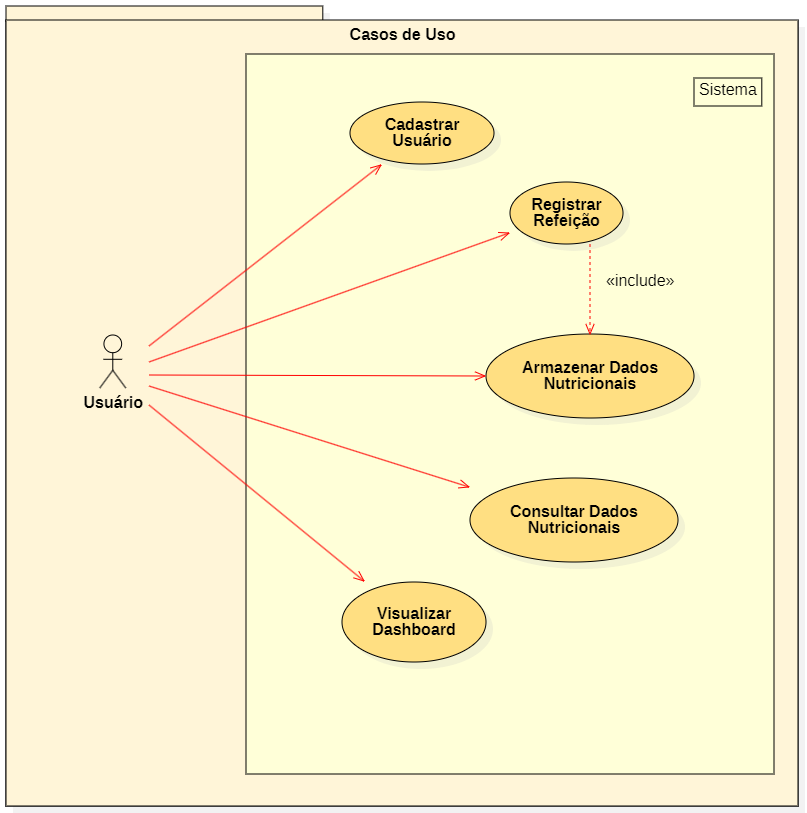
\includegraphics[width=0.8\textwidth]{Figuras/casos-uso-reducao.png}
    \caption{Diagrama de Casos de Uso após redução de escopo}
    \label{fig:casos-uso-reducao}
\end{figure}

\section{Cálculo do Novo Valor de Use Case Points (UCP) após Redução}

Considerando o novo valor de UUCP = 60, e mantendo os fatores técnicos (TCF) e ambientais (ECF) já calculados no Capítulo \ref{cap:8-ger-req-use-case-points}, temos:

\begin{itemize}
    \item \textbf{UUCP:} 60
    \item \textbf{TCF:} 1,055
    \item \textbf{ECF:} 0,53
\end{itemize}

O cálculo do novo valor de UCP é:

\begin{align*}
    UCP &= UUCP \times TCF \times ECF \\
    &= 60 \times 1,055 \times 0,53 \\
    &= 63,3 \times 0,53 \\
    &= 33,549 \\
    &\approx \textbf{33,5}
\end{align*}

Portanto, o novo valor de UCP após a redução de escopo é \textbf{33,5}. Considerando a estimativa de 10 horas por UCP:

\begin{itemize}
    \item \textbf{Horas estimadas:} $33,5 \times 10 = 335$
\end{itemize}

Esse resultado demonstra que a redução de escopo atingiu e superou a meta de redução de pelo menos 30\% no custo do projeto.

\section{Considerações Finais}

A priorização e redução de requisitos são etapas críticas para garantir que o sistema atenda às necessidades essenciais dos usuários, mantendo a viabilidade do projeto. A técnica de Use Case Points permitiu uma análise objetiva do custo e da complexidade dos casos de uso, facilitando a tomada de decisão sobre quais funcionalidades manter no escopo inicial.

A redução de 30\% no custo foi alcançada com a remoção de casos de uso desejáveis e importantes, preservando as funcionalidades essenciais para o funcionamento do sistema. Essa abordagem garante que o projeto possa ser implementado de forma eficiente, com foco nas necessidades mais críticas dos usuários.   




\chapter{Conclusões}\label{cap:10-conclusoes}

   

% ELEMENTOS PÓS-TEXTUAIS
%---------- Referencias ----------
\clearpage % this is need for add +1 to pageref of bibstart used in 'ficha catalografica'.
\label{bibstart}
\bibliography{referencias} % geracao automatica das referencias a partir do arquivo referencias.bib
\label{bibend}


% %---------- APÊNDICES (opcionais) ----------
% \apendice
% \chapter{APÊNDICE A - APÊNDICE COM UM ITEM APENAS}\label{cap-apendice-a}

% \chapter{APÊNDICE B - NOME DO APÊNDICE COM MAIS DE 1 ITEM}\label{cap-apendice-b}
% \section{PRIMEIRO ITEM - APÊNDICE B.1}

% \newpage
% \section{SEGUNDO ITEM - APÊNDICE B.2}

% Use o comando {\ttfamily \textbackslash apendice} e depois comandos {\ttfamily \textbackslash chapter\{\}}
% para gerar t\'itulos de ap\^en-dices.


% % ---------- ANEXOS (opcionais) ----------
% \anexo
% \chapter{Nome do Anexo}

% Use o comando {\ttfamily \textbackslash anexo} e depois comandos {\ttfamily \textbackslash chapter\{\}}
% para gerar t\'itulos de anexos.


% --------- Ordenacao Afabetica da Lista de siglas --------
%\textbf{* Observa\c{c}\~oes:} a ordenacao alfabetica da lista de siglas ainda nao eh realizada de forma automatica, porem
% eh possivel se de realizar isto manualmente. Duas formas:
%
% ** Primeira forma)
%    A ordenacao eh feita com o auxilio do comando 'sort', disponivel em qualquer
% sistema Linux e UNIX, e tambem em sistemas Windows se instalado o coreutils (http://gnuwin32.sourceforge.net/packages/coreutils.htm)
% comandos para compilar e ordenar, supondo que seu arquivo se chame 'dissertacao.tex':
%
%      $ latex dissertacao
%      $ bibtex dissertacao && latex dissertacao
%      $ latex dissertacao
%      $ sort dissertacao.lsg > dissertacao.lsg.tmp
%      $ mv dissertacao.lsg.tmp dissertacao.lsg
%      $ latex dissertacao
%      $ dvipdf dissertacao.dvi
%
%
% ** Segunda forma)
%\textbf{Sugest\~ao:} crie outro arquivo .tex para siglas e utilize o comando \sigla{sigla}{descri\c{c}\~ao}.
%Para incluir este arquivo no final do arquivo, utilize o comando \input{arquivo.tex}.
%Assim, Todas as siglas serao geradas na ultima pagina. Entao, devera excluir a ultima pagina da versao final do arquivo
% PDF do seu documento.


%-------- Citacoes ---------
% - Utilize o comando \citeonline{...} para citacoes com o seguinte formato: Autor et al. (2011).
% Este tipo de formato eh utilizado no comeco do paragrafo. P.ex.: \citeonline{autor2011}

% - Utilize o comando \cite{...} para citacoeses no meio ou final do paragrafo. P.ex.: \cite{autor2011}



%-------- Titulos com nomes cientificos (titulo, capitulos e secoes) ----------
% Regra para escrita de nomes cientificos:
% Os nomes devem ser escritos em italico, 
%a primeira letra do primeiro nome deve ser em maiusculo e o restante em minusculo (inclusive a primeira letra do segundo nome).
% VEJA os exemplos abaixo.
% 
% 1) voce nao quer que a secao fique com uppercase (caixa alta) automaticamente:
%\section[nouppercase]{\MakeUppercase{Estudo dos efeitos da radiacao ultravioleta C e TFD em celulas de} {\textit{Saccharomyces boulardii}}
%
% 2) por padrao os cases (maiusculas/minuscula) sao ajustados automaticamente, voce nao precisa usar makeuppercase e afins.
% \section{Introducao} % a introducao sera posta no texto como INTRODUCAO, automaticamente, como a norma indica.

%\balance
\end{document}
